\section{The black-box problem of modern AI systems}

\begin{frame}{The black-box problem of modern AI systems}
    \begin{tikzpicture}
        \node[] at (-7, -3.25) {};
        \node[] at (7, 3.25) {};

        \only<1-4>{
            \node[fill=gray!80, minimum width=6cm, minimum height=6.5cm, rounded corners=0.1cm, text=white, font=\systemfont, text depth=6cm, alt=<4>{draw=red}{draw=black}, thick] (multi) at (-0.6, 0.2) {
                Multimodal ANN
            };

            \node[] (ehr) at ($ (multi) - (1.85, -1.8) $) {
                \encoder{EHR encoder}{ehrenc}
            };
            \node[] (mri) at ($ (multi) - (1.85, 0.2) $) {
                \encoder{MRI encoder}{mrienc}
            };
            \node[] (bio) at ($ (multi) - (1.85, 2.2) $) {
                \encoder{Bio encoder}{bioenc}
            };


            \node[anchor=east, inner sep=0pt, alt=<3>{draw=red}{draw=none}, thick] (input2) at ($ (ehr.west) - (1, 0.2) $) {
                {\Huge{\emoji{spiral-notepad}}}
            };
            \draw[-stealth] (input2) -- ($ (ehr.west) - (-0.1, 0.2) $);
            \node[anchor=east, inner sep=0pt, alt=<3>{draw=red}{draw=black}, thick] (input) at ($ (mri.west) - (1, 0.2) $) {
                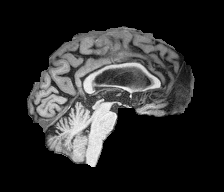
\includegraphics[width=1.5cm]{data/mri_sagittal.png}
            };
            \draw[-stealth] (input) -- ($ (mri.west) - (-0.1, 0.2) $);
            \node[anchor=east, inner sep=0pt, alt=<3>{draw=red}{draw=none}, thick] (input3) at ($ (bio.west) - (1, 0.2) $) {
                {\Huge{\emoji{microscope}}}
            };
            \draw[-stealth] (input3) -- ($ (bio.west) - (-0.1, 0.2) $);

            \neuron{n00}{($ (multi.south) + (0, 1.85) + (-0.5*\hsep, -2*\vsep) $)}
            \neuron{n01}{($ (n00) + (0, 2*\vsep) $)}
            \neuron{n02}{($ (n00) + (0, 4*\vsep) $)}
            \neuron{n03}{($ (n00) + (0, 6*\vsep) $)}
            \neuron{n04}{($ (n00) + (0, 8*\vsep) $)}
            \neuron{n10}{($ (n00) + (\hsep, 1*\vsep) $)}
            \neuron{n11}{($ (n00) + (\hsep, 3*\vsep) $)}
            \neuron{n12}{($ (n00) + (\hsep, 5*\vsep) $)}
            \neuron{n13}{($ (n00) + (\hsep, 7*\vsep) $)}

            \neuron{n20}{($ (n00) + (2*\hsep, 2*\vsep) $)}
            \neuron{n21}{($ (n00) + (2*\hsep, 4*\vsep) $)}
            \neuron{n22}{($ (n00) + (2*\hsep, 6*\vsep) $)}

            \neuron{n30}{($ (n00) + (3*\hsep, 3*\vsep) $)}
            \neuron{n31}{($ (n00) + (3*\hsep, 5*\vsep) $)}

            \neuron{n40}{($ (n00) + (4*\hsep, 4*\vsep) $)}

            \foreach \j in {0,...,4} {
                \draw[black, opacity=\edgeopacity] ($ (ehr.east) - (0.77, -0.04) $) -- (n0\j);
                \draw[black, opacity=\edgeopacity] ($ (ehr.east) - (0.77, 0.46) $) -- (n0\j);
                \draw[black, opacity=\edgeopacity] ($ (mri.east) - (0.77, -0.04) $) -- (n0\j);
                \draw[black, opacity=\edgeopacity] ($ (mri.east) - (0.77, 0.46) $) -- (n0\j);
                \draw[black, opacity=\edgeopacity] ($ (bio.east) - (0.77, -0.04) $) -- (n0\j);
                \draw[black, opacity=\edgeopacity] ($ (bio.east) - (0.77, 0.46) $) -- (n0\j);
                \foreach \k in {0,...,3} {
                    \draw[black, opacity=\edgeopacity] (n0\j) -- (n1\k);
                }
            }
            \foreach \j in {0,...,3} {
                \foreach \k in {0,...,2} {
                    \draw[black, opacity=\edgeopacity] (n1\j) -- (n2\k);
                }
            }
            \foreach \j in {0,...,2} {
                \foreach \k in {0,...,1} {
                    \draw[black, opacity=\edgeopacity] (n2\j) -- (n3\k);
                }
            }
            \draw[black, opacity=\edgeopacity] (n30) -- (n40);
            \draw[black, opacity=\edgeopacity] (n31) -- (n40);
            \draw[black, opacity=\edgeopacity] (n40) -- ($ (multi.south east) + (0, 2.85) $);

            \node[anchor=west, font=\small, align=left, alt=<2-3>{draw=red}{draw=none}, thick] (output) at ($ (multi.south east) + (1, 2.85) $) {Clinical\\prediction};
            \draw[-stealth] ($ (multi.south east) + (0, 2.85) $) -- (output);
        }
        \only<5-8>{
            \node[fill=gray!80, minimum width=4cm, minimum height=2.9cm, rounded corners=0.1cm, text=white, draw=black, font=\systemfont, anchor=south, text depth=2.4cm] (model) at (0, 0) {
                Artificial neural network
            };
            \only<7->{
                \node[anchor=east, inner sep=0pt, draw=black] (input) at (-3, 1.25) {
                    \only<7>{%
                        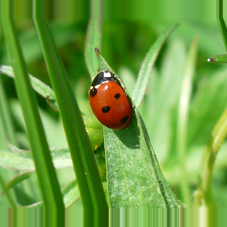
\includegraphics[width=2.5cm]{data/ladybug.png}
                    }%
                    \only<8>{%
                        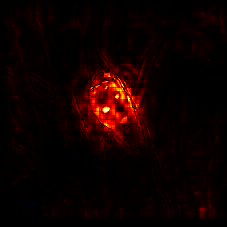
\includegraphics[width=2.5cm]{data/ladybug_explanation.png}
                    }%
                };
                \draw[alt=<8>{draw=red, stealth-}{draw=black, -stealth}] (input) -- ($ (model.west) - (0, 0.2175) $);
            }
            \only<7->{
                \node[anchor=west, alt=<8>{text=red}{text=black}] (output) at (3, 1.25) {$\text{ladybug}$};
                \draw[
                    alt=<8>{draw=red, stealth-}{draw=black, -stealth}
                ] ($ (model.south east) + (0, 1.25) $) -- (output);
            }
            \only<5-6>{
                \node[circle, draw=black, fill=uiogreen, minimum size=0.5cm] (neuron) at ($ (model.south) - (0, 1.5) $) {};

                \node[anchor=east, font=\scriptsize] (x1) at ($ (neuron) - (0.75, -0.5) $) {$\text{input}_1$};
                \node[anchor=east, font=\scriptsize] (x2) at ($ (neuron) - (0.75, 0) $) {$\text{input}_2$};
                \node[anchor=east, font=\scriptsize] (x3) at ($ (neuron) - (0.75, 0.5) $) {$\text{input}_3$};

                \node[anchor=west, font=\scriptsize] (y) at ($ (neuron) + (0.75, 0) $) {$\text{output}$};

                \draw[-stealth] (x1) -- (neuron);
                \draw[-stealth] (x2) -- (neuron);
                \draw[-stealth] (x3) -- (neuron);
                \draw[-stealth] (neuron) -- (y);

                \node[font=\small] at ($ (neuron) + (0, 1) $) {
                    Artificial neuron
                };
            }
            \only<6>{
                \node[font=\small] at ($ (neuron.south) - (0, 1.25) $) {
                    $\text{output}=\text{max}(0, \text{input}_1*w_1+\text{input}_2*w_2+\text{input}_3*w_3)$
                };
            }
            \only<5-6>{
                \neuron{n00}{($ (model.south) + (0, 1.25) + (-2*\hsep, -2*\vsep) $)}
                \neuron{n01}{($ (n00) + (0, \vsep) $)}
                \neuron{n02}{($ (n00) + (0, 2*\vsep) $)}
                \neuron{n03}{($ (n00) + (0, 3*\vsep) $)}
                \neuron{n04}{($ (n00) + (0, 4*\vsep) $)}
            }
            \only<7>{
                \neuron[uiogreen!60]{n00}{($ (model.south) + (0, 1.25) + (-2*\hsep, -2*\vsep) $)}
                \neuron[uiogreen!30]{n01}{($ (n00) + (0, \vsep) $)}
                \neuron[uiogreen!50!black]{n02}{($ (n00) + (0, 2*\vsep) $)}
                \neuron[uiogreen!70]{n03}{($ (n00) + (0, 3*\vsep) $)}
                \neuron[uiogreen!35!black]{n04}{($ (n00) + (0, 4*\vsep) $)}
            }
            \only<8->{
                \neuron[red!25!black]{n00}{($ (model.south) + (0, 1.25) + (-2*\hsep, -2*\vsep) $)}
                \neuron[red!90!black]{n01}{($ (n00) + (0, \vsep) $)}
                \neuron[yellow!15!red]{n02}{($ (n00) + (0, 2*\vsep) $)}
                \neuron[red!99!black]{n03}{($ (n00) + (0, 3*\vsep) $)}
                \neuron[red!10!black]{n04}{($ (n00) + (0, 4*\vsep) $)}
            }

            \only<5-6>{
                \neuron{n10}{($ (n00) + (\hsep, 0.5*\vsep) $)}
                \neuron{n11}{($ (n00) + (\hsep, 1.5*\vsep) $)}
                \neuron{n12}{($ (n00) + (\hsep, 2.5*\vsep) $)}
                \neuron{n13}{($ (n00) + (\hsep, 3.5*\vsep) $)}
            }
            \only<7>{
                \neuron[uiogreen!80!black]{n10}{($ (n00) + (\hsep, 0.5*\vsep) $)}
                \neuron[uiogreen!20]{n11}{($ (n00) + (\hsep, 1.5*\vsep) $)}
                \neuron[uiogreen!50]{n12}{($ (n00) + (\hsep, 2.5*\vsep) $)}
                \neuron[uiogreen!90]{n13}{($ (n00) + (\hsep, 3.5*\vsep) $)}
            }
            \only<8->{
                \neuron[red!55!black]{n10}{($ (n00) + (\hsep, 0.5*\vsep) $)}
                \neuron[yellow!20!red]{n11}{($ (n00) + (\hsep, 1.5*\vsep) $)}
                \neuron[yellow!90!red]{n12}{($ (n00) + (\hsep, 2.5*\vsep) $)}
                \neuron[red!7!black]{n13}{($ (n00) + (\hsep, 3.5*\vsep) $)}
            }

            \only<5-6>{
                \neuron{n20}{($ (n00) + (2*\hsep, \vsep) $)}
                \neuron{n21}{($ (n00) + (2*\hsep, 2*\vsep) $)}
                \neuron{n22}{($ (n00) + (2*\hsep, 3*\vsep) $)}
            }
            \only<7>{
                \neuron[uiogreen!80!black]{n20}{($ (n00) + (2*\hsep, \vsep) $)}
                \neuron[uiogreen!55!black]{n21}{($ (n00) + (2*\hsep, 2*\vsep) $)}
                \neuron[uiogreen!45]{n22}{($ (n00) + (2*\hsep, 3*\vsep) $)}
            }
            \only<8->{
                \neuron[red!90!black]{n20}{($ (n00) + (2*\hsep, \vsep) $)}
                \neuron[red!30!black]{n21}{($ (n00) + (2*\hsep, 2*\vsep) $)}
                \neuron[yellow!70!red]{n22}{($ (n00) + (2*\hsep, 3*\vsep) $)}
            }

            \only<5-6>{
                \neuron{n30}{($ (n00) + (3*\hsep, 1.5*\vsep) $)}
                \neuron{n31}{($ (n00) + (3*\hsep, 2.5*\vsep) $)}
            }
            \only<7>{
                \neuron[uiogreen!70]{n30}{($ (n00) + (3*\hsep, 1.5*\vsep) $)}
                \neuron[uiogreen!33]{n31}{($ (n00) + (3*\hsep, 2.5*\vsep) $)}
            }
            \only<8->{
                \neuron[yellow!40!red]{n30}{($ (n00) + (3*\hsep, 1.5*\vsep) $)}
                \neuron[red!65!black]{n31}{($ (n00) + (3*\hsep, 2.5*\vsep) $)}
            }

            \only<5-6>{
                \neuron{n40}{($ (n00) + (4*\hsep, 2*\vsep) $)}
            }
            \only<7>{
                \neuron[uiogreen!20]{n40}{($ (n00) + (4*\hsep, 2*\vsep) $)}
            }
            \only<8->{
                \neuron[red]{n40}{($ (n00) + (4*\hsep, 2*\vsep) $)}
            }

            \foreach \j in {0,...,4} {
                \draw[draw=black, alt=<8>{draw=red}{}, opacity=\edgeopacity] ($ (model.west) - (0, 0.2175) $) -- (n0\j);
            }

            \foreach \j in {0,...,4} {
                \foreach \k in {0,...,3} {
                    \draw[draw=black, alt=<8>{draw=red}{}, opacity=\edgeopacity] (n0\j) -- (n1\k);
                }
            }
            \foreach \j in {0,...,3} {
                \foreach \k in {0,...,2} {
                    \draw[draw=black, alt=<8>{draw=red}{}, opacity=\edgeopacity] (n1\j) -- (n2\k);
                }
            }
            \foreach \j in {0,...,2} {
                \foreach \k in {0,...,1} {
                    \draw[draw=black, alt=<8>{draw=red}{}, opacity=\edgeopacity] (n2\j) -- (n3\k);
                }
            }
            \draw[alt=<8>{draw=red}{draw=black}, opacity=\edgeopacity] (n30) -- (n40);
            \draw[alt=<8>{draw=red}{draw=black}, opacity=\edgeopacity] (n31) -- (n40);
            \draw[alt=<8>{draw=red}{draw=black}, opacity=\edgeopacity] (n40) -- ($ (model.south east) + (0, 1.25) $);
        }
        \only<9>{
            \inputside{-4.5}{-0.2175}{1.5cm}
            \cnnarrow{(input.east)}{($ (input.center) + (3, 0) $)}{black}
            \cnn{-2.7}{-0.2175}{0.1}{0.15}{uiogreen}{1}
            \node[anchor=west, align=left, font=\normalfont\linespread{0.9}\selectfont] (output1) at ($ (3.55, -0.2175) + (0, 0.5) $) {Dementia\\patient};
            \cnnarrow{($ (output1.west) - (1, 0.5) $)}{($ (output1.west) + (0.1, 0) $)}{black}
            \node[anchor=west, align=left, font=\normalfont\linespread{0.9}\selectfont] (output2) at ($ (3.55, -0.2175) - (0, 0.5) $) {Healthy\\control};
            \cnnarrow{($ (output2.west) - (1, -0.5) $)}{($ (output2.west) + (0.1, 0) $)}{black}
        }
        \only<10>{
            \heatmapside{-4.5}{-0.2175}{1.5cm}
            \lrparrow{($ (input.center) + (3, 0) $)}{(input.east)}{black}
            \lrp{-2.7}{-0.2175}{0.1}{0.15}
            \node[anchor=west, align=left, font=\normalfont\linespread{0.9}\selectfont] (output1) at ($ (3.55, -0.2175) + (0, 0.5) $) {Dementia\\patient};
            \lrparrow{($ (output1.west) + (0.1, 0) $)}{($ (output1.west) - (1, 0.5) $)}{black}
        }
    \end{tikzpicture}
\end{frame}

\begin{frame}{Explainable AI and dementia}
    \begin{tikzpicture}
        \node[] at (-7, -3.25) {};
        \node[] at (7, 3.25) {};

        \only<1>{
            \node[
				minimum height=0.41\textwidth,
				minimum width=0.32\textwidth,
				fill=black,
                anchor=west
			] (box1) at (-6.8, 0) {};
			\node[anchor=south] at (box1.south) {
				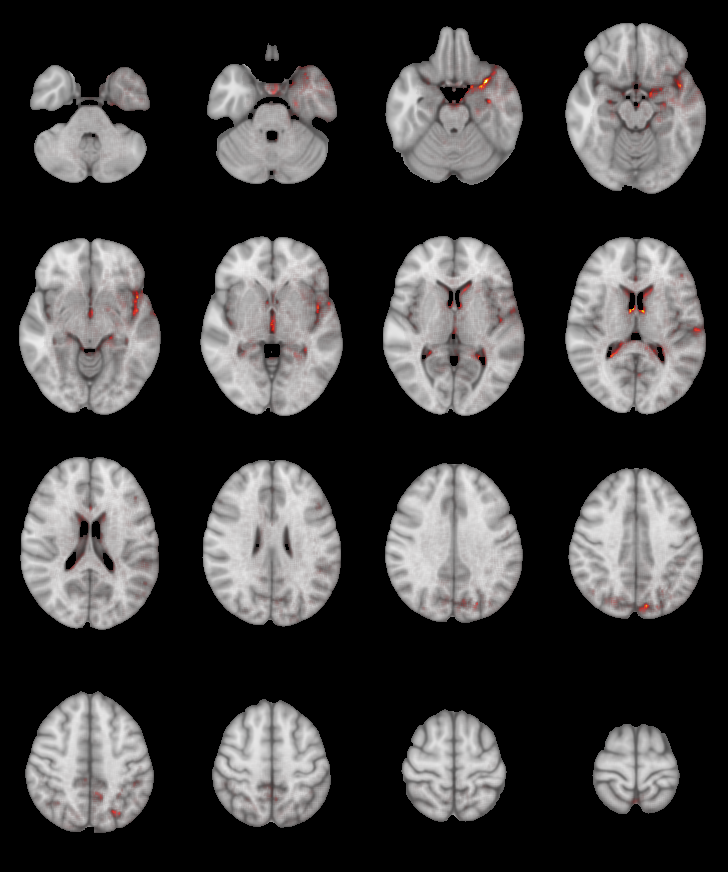
\includegraphics[width=0.31\textwidth]{data/subject1.png}
			};
			\node[anchor=north,inner sep=2pt, text=white, font=\footnotesize] at (box1.north) {Pasient 1};

			\node
				[minimum height=0.41\textwidth,
				minimum width=0.32\textwidth,
				fill=black,
				anchor=west
			] (box2) at ($ (box1.east) + (0.05,0) $) {};
			\node[anchor=south] at (box2.south) {
				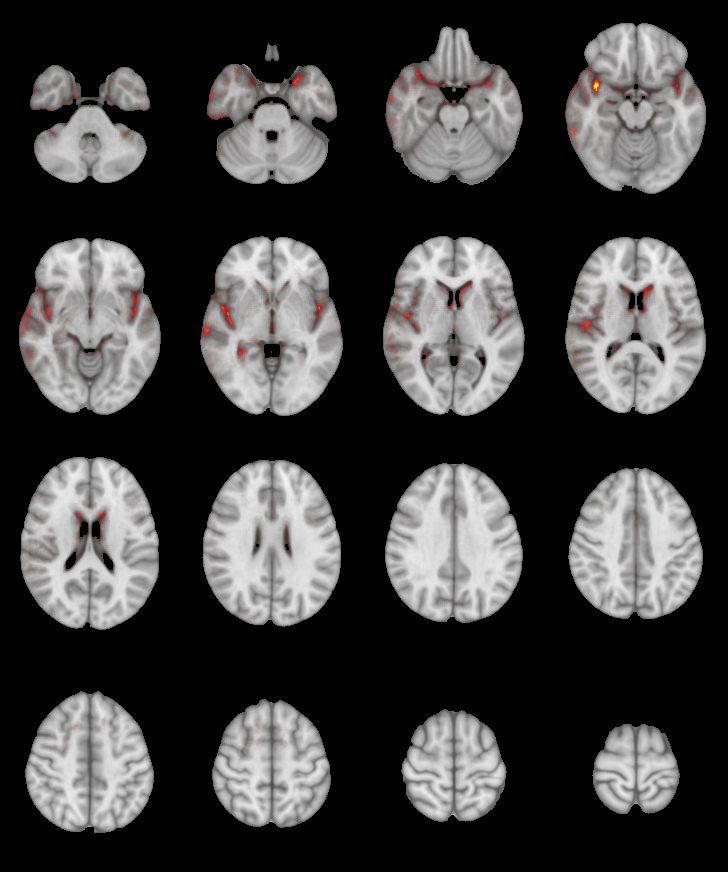
\includegraphics[width=0.31\textwidth]{data/subject2.png}
			};
			\node[anchor=north,inner sep=3pt, text=white, font=\footnotesize] at (box2.north) {Pasient 2};

			\node
				[minimum height=0.41\textwidth,
				minimum width=0.32\textwidth,
				fill=black,
				anchor=west
			] (box3) at ($ (box2.east) + (0.05,0) $) {};
			\node[anchor=south] at (box3.south) {
				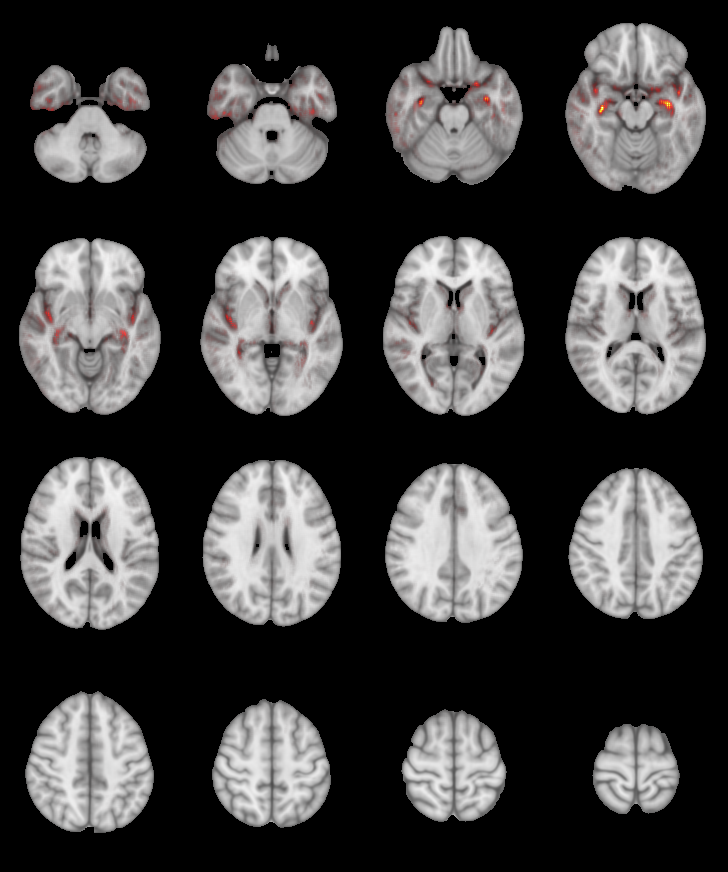
\includegraphics[width=0.31\textwidth]{data/subject3.png}
			};
			\node[anchor=north,inner sep=3pt, text=white, font=\footnotesize] at (box3.north) {Pasient 3};
        }
        \only<2-3>{
            \node[label={[text depth=0]above:Forklarbar KI}] at (-2.5, 0) {
				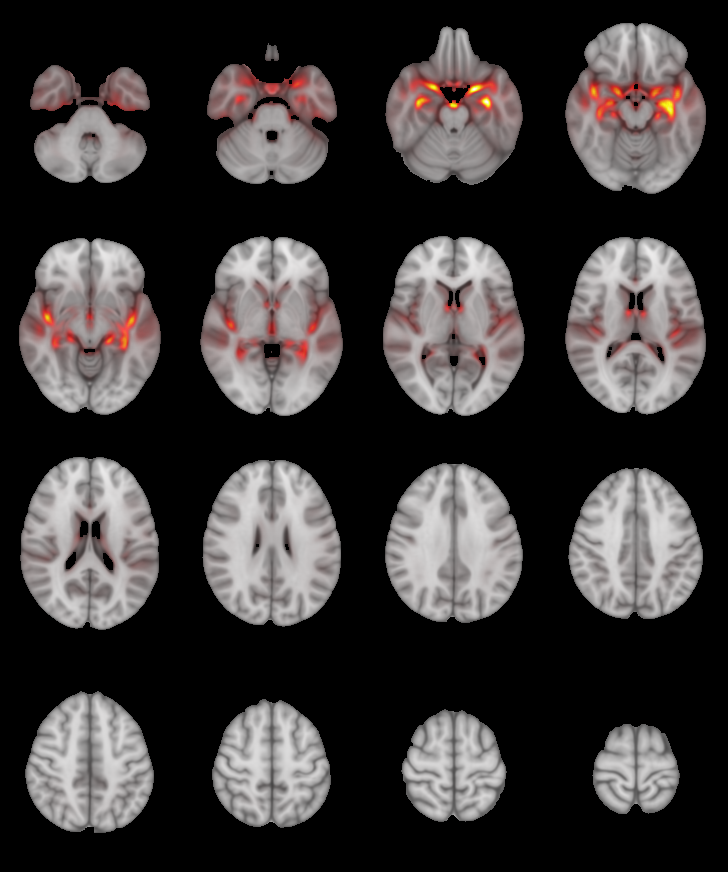
\includegraphics[width=0.31\textwidth]{data/dementia.png}
			};
        }
        \only<3>{
			\node[label={[text depth=0]above:Mennesker}] at (2.5, 0) {
				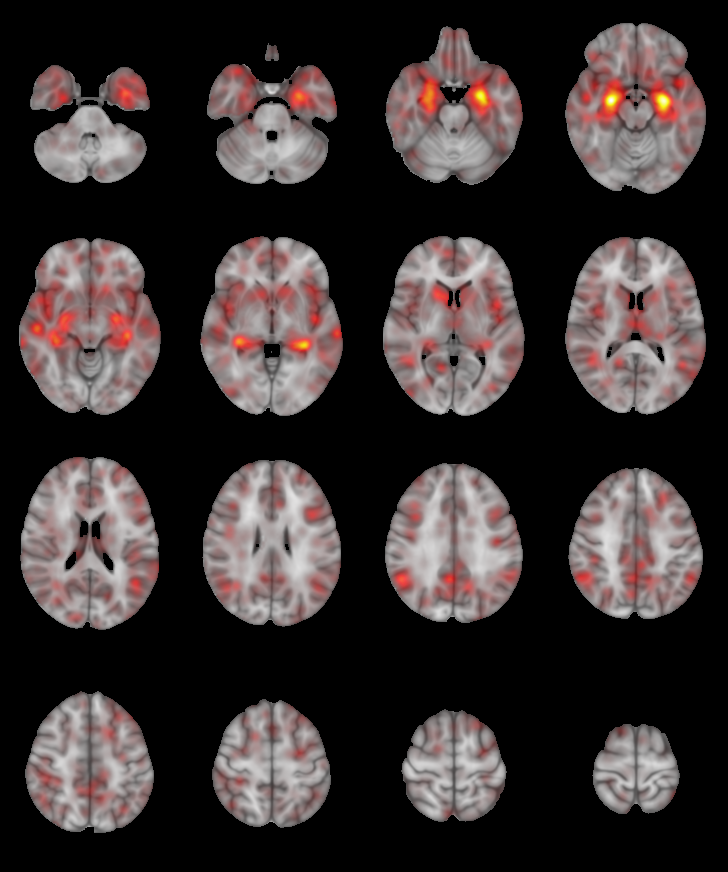
\includegraphics[width=0.31\textwidth]{data/ALE.png}
			};
        }
    \end{tikzpicture}
\end{frame}

\begin{frame}{Explainable AI and multimodality}
    \begin{tikzpicture}
        \node[] at (-7, -3.25) {};
        \node[] at (7, 3.25) {};

        \only<1>{
            \node[inner sep=0pt, draw=black] at (0, 1.5) {
                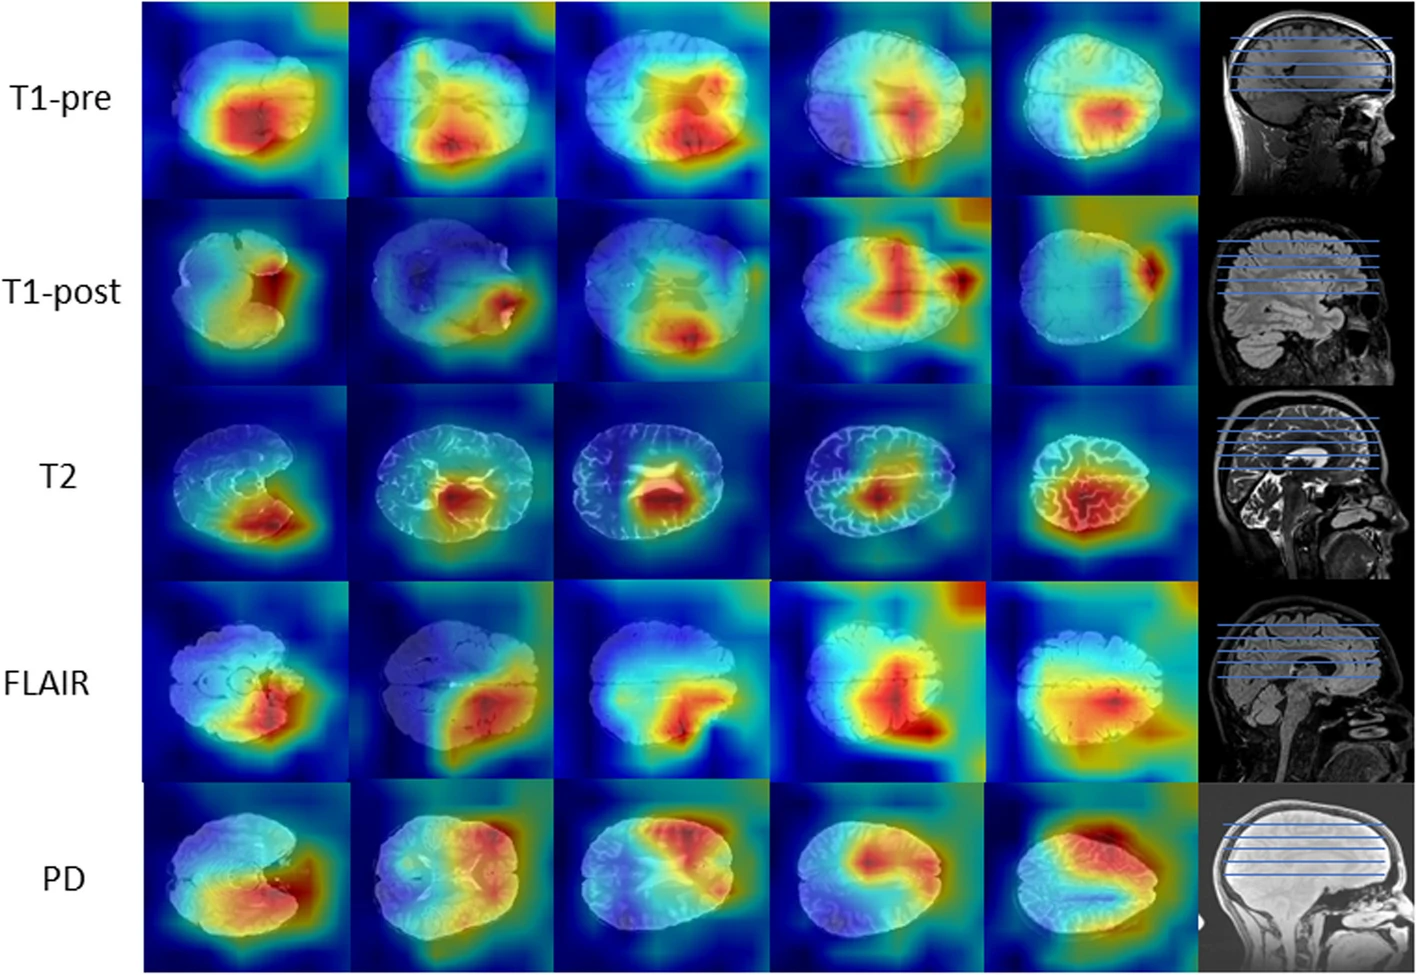
\includegraphics[width=5cm]{data/zhang_mri_weights.png}
            };
            \node[inner sep=0pt, draw=black] at (0, -2) {
                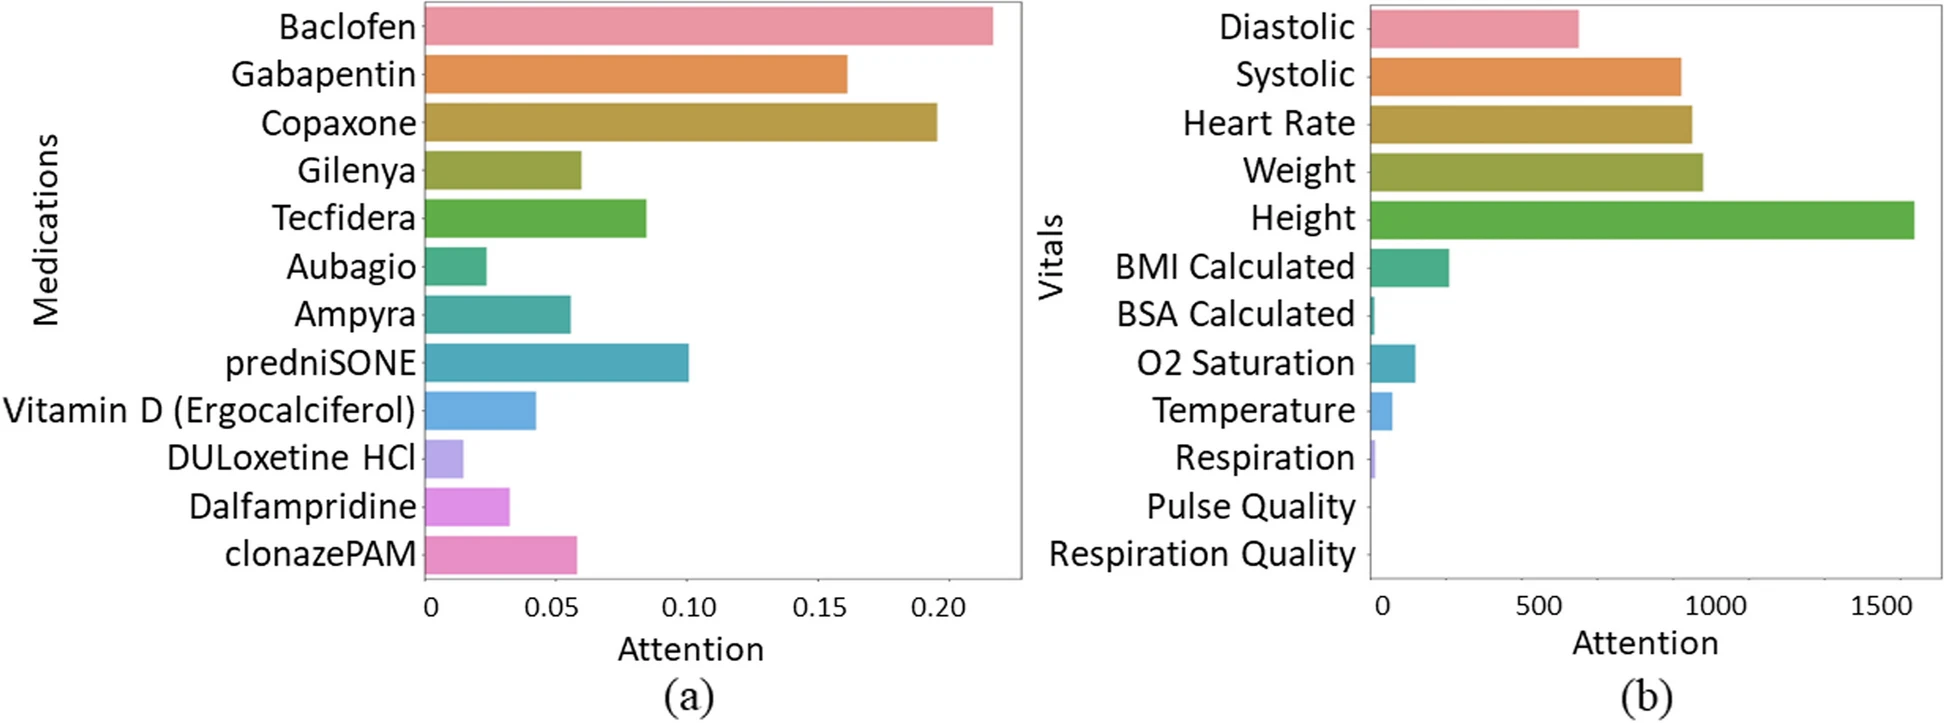
\includegraphics[width=7cm]{data/zhang_medication_weights.png}
            };
        }
        \only<2>{
            \node[inner sep=0pt, draw=black] at (0, 0) {
                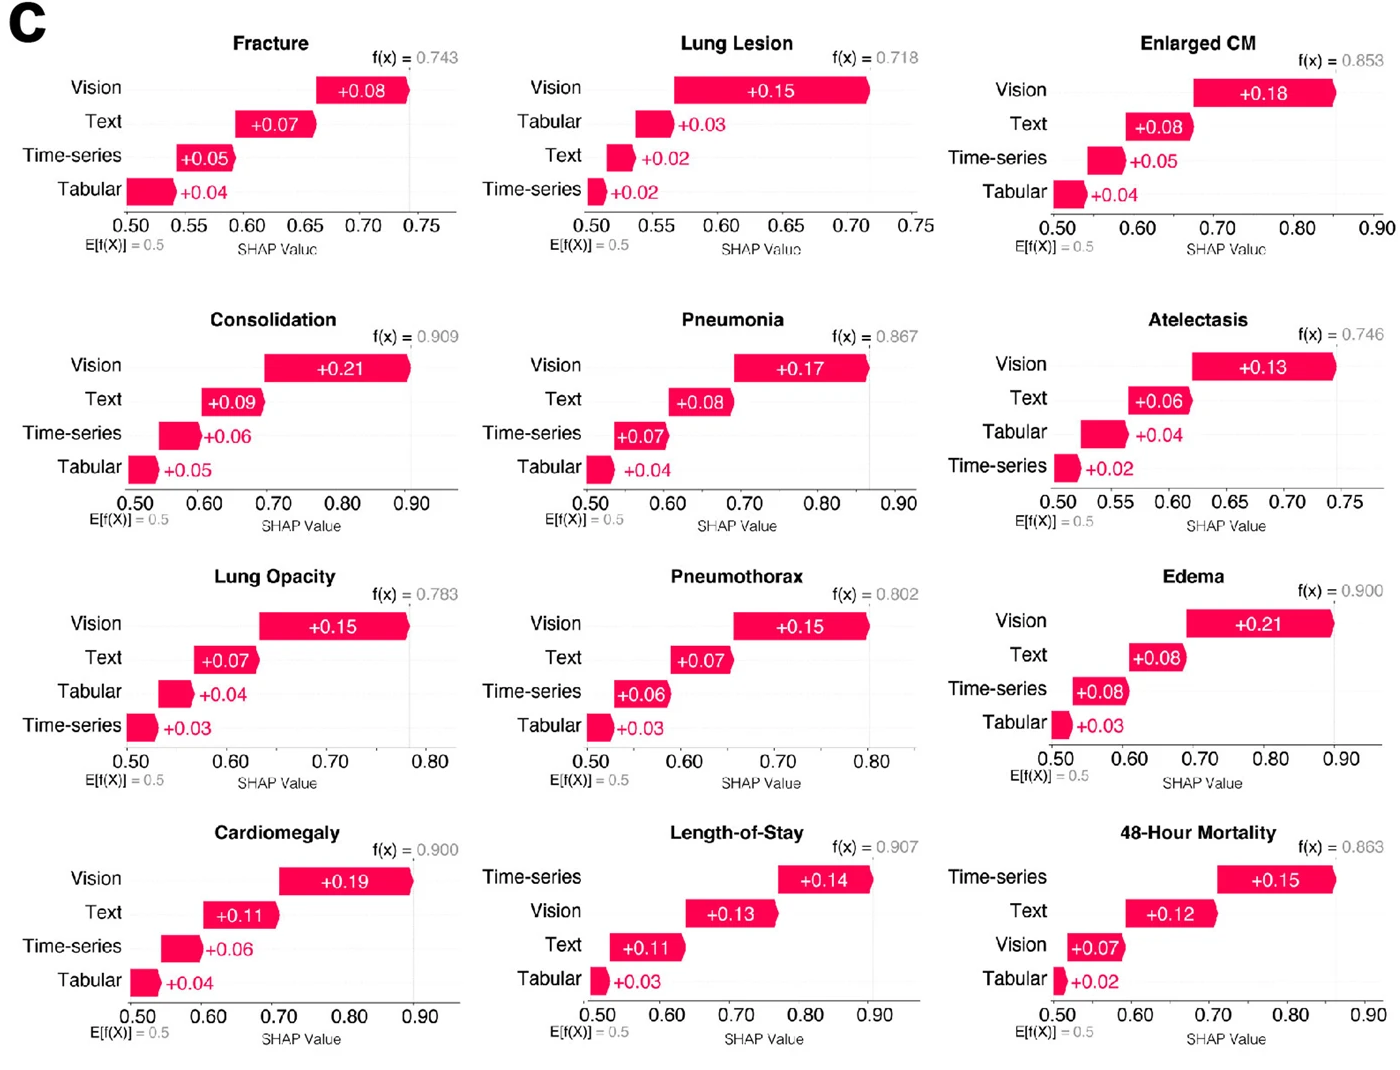
\includegraphics[width=8cm]{data/soenksen.png}
            };
        }

    \end{tikzpicture}
\end{frame}

\begin{frame}{Summary}
    \begin{itemize}
        \item Deep learning is transforming many fields, enabling complex modelling of diverse, unstructured data.
        \item Multimodal AI requires decisions about how and when to combine information.
        \begin{itemize}
            \item Late fusion: Information is merged after the most complex modelling
            \item Early fusion: Information is merged before the most complex modelling
            \item Intermediate fusion: Information is merged as a part of the most complex modelling
        \end{itemize}
        \item Multimodal AI systems may enable clinical predictions with an accuracy surpassing what is currently possible, but explainability remains a challenge
        \begin{itemize}
            \item Methods are emerging to alleviate these problems, at least partially
        \end{itemize}
    \end{itemize}
\end{frame}